\documentclass{standalone}

\usepackage{tikz}
    \usetikzlibrary{arrows.meta}
    \usetikzlibrary{calc}
    \usetikzlibrary{decorations.pathmorphing}

\tikzset{
    bluearrow/.style={
        blue!25,
        -{Kite[length=2.5mm]}, 
        line width=0.5mm,},
    greensq/.style={
        green,
        fill=green!20, 
        line width=0.4mm,},
    redsq/.style={
        red,
        fill=red!20, 
        line width=0.4mm,},
    }
    
\begin{document}
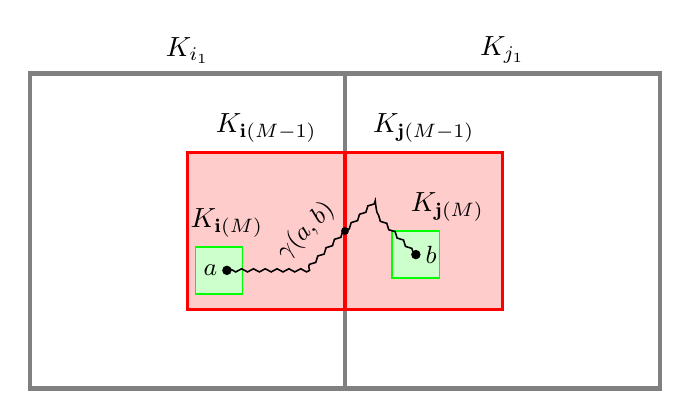
\begin{tikzpicture}
    % \draw[help lines] (0,0) grid (15,3);
    \draw[black!50, line width=0.6mm] 
        (0,0)rectangle+(4,4)
        (4,0) rectangle+(4,4);
    \draw[red, fill=red!20, line width=0.4mm] 
        (2,1) rectangle+(2,2)
        (4,1) rectangle+(2,2);
    \draw[green, fill=green!20, line width=0.2mm,] 
        (4.6,2) rectangle+(0.6,-0.6)
        (2.1,1.2) rectangle+(0.6,0.6);
    \fill[black] 
        (2.5,1.5) circle (0.6mm)
        (4,2) circle (0.5mm)
        (4.9,1.7) circle (0.6mm);
    \draw[line width=0.2mm, decorate, decoration={coil,aspect=0,segment length=1.5mm,amplitude=0.2mm}]
        (2.5,1.5)--(3.5,1.5)--(4,2)--(4.3,2.3)--(4.9,1.7);
    \node[shift={(2,4)}, above]
        {$K_{i_1}$};
    \node[shift={(6,4)}, above]
        {$K_{j_1}$};
    \node[shift={(3,3)}, above]
        {$K_{{\bf i}(M-1)}$};
    \node[shift={(5,3)}, above]
        {$K_{{\bf j}(M-1)}$};
    \node[shift={(2.5,1.8)},above]
        {$K_{{\bf i}(M)}$};
    \node[shift={(5.3,2)}, above]
        {$K_{{\bf j}(M)}$};
    \node[shift={(2.5,1.5)},left]{\small$a$};
    \node[shift={(4.9,1.7)}, right]{\small$b$};
    \node[shift={(3.5,2)},rotate=45]{\small$\gamma(a,b)$};
    

\end{tikzpicture}
\end{document}